
\chapter{Results}
\label{chap:res}

This chapter covers the findings of the experiments described in \RefChap{chap:method}. These experiments aim at quantifying the performance of the RepNet algorithm in both simple and more complex scenarios while demonstrating its strong points, as well as shortcomings. 
The chapter follows the following structure: in \RefSec{sec:feat}, the fundamental properties that differentiate the RepNet framework from other MDP-derived frameworks are presented. \RefSec{sec:adapt} covers the ability of the algorithm to quickly adapt to changes in the behavior of other agents. \RefSec{sec:large} presents the results related to the two large-scale experiments. Finally, \RefSec{sec:summa} summarizes the results.

\section{The properties of the RepNet framework}
\label{sec:feat}
In this section, the concepts of \textit{action distribution}, \textit{image}, \textit{reputation}, and \textit{directed actions}, as well as these concepts' effects on RepNet agents' behavior, are quantified. The results of two sets of experiments are presented hereafter. The first set of experiments covers  \textit{action distribution}, \textit{image}, \textit{reputation} in the absence of \textit{directed actions}, while the second set covers the same properties in their presence.

\subsection{Testing action distribution, image, and reputation}
The \textit{action distribution}, \textit{image}, and \textit{reputation} of agent $A$ are tracked throughout the experiment, which is made up of 5 runs, of which the average one is analyzed hereafter. As such, \RefFig{subfig:paccept} shows the evolution of agent $A$'s action distribution for target agent $B$ in state $s = 2$ (the state in which $B$ is aware of the trade offer made by agent $A$, which has done a good deed prior to the offer, see \RefFig{fig:ex1}). \RefFig{subfig:image} displays the image $B$ has of $A$ and vice versa, according to $A$.
\RefFig{subfig:rep} shows the reputation of $A$ and $B$, according to $A$. Finally, \RefFig{subfig:freq} displays the tangible effects of these variables on $A$'s behavior. Concretely it shows the evolution of the frequency at which $A$ makes trade offers. Note that to maintain clarity, a shorthand notation for the reputation is used in this chapter, that is,
\begin{align}
    REP_g(h,Img_g) = REP_g(h) \,\,\,   \forall g, h \in \mathcal{G}.
\end{align}

In the first 20 time-steps, $B$ refuses each trade offer. Agent $A$ is able to pick up on this via the action distribution. As a consequence, it quickly reduces the frequency at which it attempts to trade with $B$. $A$'s image of $B$, and, by extension, $B$'s reputation (\RefDef{def:repnew}) quickly drop alongside. Interestingly, $A$'s self-reputation decreases in a similar fashion. In fact, $B$ refusing to trade with $A$ can be explained as having two effects on $A$'s perception of the network, both following from the current mathematical definition of reputation (\RefDef{def:repnew}):
\begin{itemize}
    \item $B$ is an unreliable agent and should, therefore, have a poor reputation. The image $A$ has of $B$ decreases, and consequently, so does $B$'s reputation.
    \item $B$ refuses to trade with $A$ because it believes $A$ to be unreliable. $A$ must adapt its self-reputation based on the evidence it is provided with. In this case, the evidence points towards the fact that $A$ might be seen as unreliable in the network, which only includes $B$. 
\end{itemize}
The similarity between $A$'s and $B$'s reputations can be further explained by the fact that the network is made up of only two agents. As such, the evidence provided to $A$ is insufficient for it to make up its mind as to the cause of $B$'s changes in behavior.



In the 60 following time-steps, $B$ is asked to change its behavior and accept each trade offer. Hesitant at first, $A$ gradually increases the frequency at which it attempts to trade with $B$. $B$'s reputation, as well as $A$'s self-reputation, are positively impacted by $B$'s change of behavior. The same two-effect explanation can be applied to explain the increase of both agents' reputations.

Finally, $B$ reverts back to its old behavior during the final 20 steps. Again, Agent $A$ is able to pick up on this change and adapt its behavior accordingly.

\begin{figure}[h]
\subfloat[Probability of $B$ accepting and refusing $A$'s trade offers, according to $A$]
{
\label{subfig:paccept}
\begin{tikzpicture}
\begin{axis}[
	xlabel=Time-steps,
	ylabel= Probability,
	title style={align=left},
	grid=both,
	minor grid style={gray!25},
	major grid style={gray!25},
	legend style={at={(1.0,1.05)},anchor=south east},
	width=0.47\linewidth,
	no marks]
\addplot[line width=1pt,solid,color=black] %
	table[x=b,y=a,col sep=comma]{CSV/tradeABaccept2u.csv};
\addlegendentry{$AD_A(B,2)(\texttt{accept})$};

\addplot[line width=1pt,dotted,color=black] %
	table[x=b,y=a,col sep=comma]{CSV/tradeABrefuse2u.csv};
\addlegendentry{$AD_A(B,2)(\texttt{refuse})$};


\draw [densely dashed, line width=1.5pt] (20,0) -- (20,1);
\draw [densely dashed, line width=1.5pt] (80,0) -- (80,1);

\end{axis}
\end{tikzpicture}
}
\quad
\subfloat[Image agents $A$ and $B$ have of each other, according to $A$]
{
\label{subfig:image}
\begin{tikzpicture}
\begin{axis}[
	xlabel=Time-steps,
	ylabel= Image,
	title style={align=left},
	grid=both,
	minor grid style={gray!25},
	major grid style={gray!25},
	legend style={at={(1.0,1.05)},anchor=south east},
	width=0.47\linewidth,
	no marks]
\addplot[line width=1pt,solid,color=black] %
	table[x=b,y=a,col sep=comma]{CSV/tradeABimgABu.csv};
\addlegendentry{$Img_A(B,A)$};

\addplot[line width=1pt,dotted,color=black] %
	table[x=b,y=a,col sep=comma]{CSV/tradeABimgBAu.csv};
\addlegendentry{$Img_A(A,B)$};

\draw [densely dashed, line width=1.5pt] (20,-2) -- (20,2);
\draw [densely dashed, line width=1.5pt] (80,-2) -- (80,2);
\end{axis}
\end{tikzpicture}
}
\caption{Undirected actions: Evolution of the action distribution and image function, according to agent $A$.}
\end{figure}

\begin{figure}[h]
\subfloat[Reputation of agents $A$ and $B$, according to $A$]
{
\label{subfig:rep}
\begin{tikzpicture}
\begin{axis}[
	xlabel=Time-steps,
	ylabel= Reputation,
	title style={align=left},
	grid=both,
	minor grid style={gray!25},
	major grid style={gray!25},
	legend style={at={(0.98,0.02)},anchor=south east},
	width=0.465\linewidth,
	no marks]
\addplot[line width=1pt,solid,color=black] %
	table[x=b,y=a,col sep=comma]{CSV/tradeABrepAu.csv};
\addlegendentry{$REP_A(A)$};

\addplot[line width=1pt,dotted,color=black] %
	table[x=b,y=a,col sep=comma]{CSV/tradeABrepBu.csv};
\addlegendentry{$REP_A(B)$};

\draw [densely dashed, line width=1.5pt] (20,-2) -- (20,2);
\draw [densely dashed, line width=1.5pt] (80,-2) -- (80,2);
\end{axis}
\end{tikzpicture}
}
\quad
\subfloat[Frequency of the trade offers made by $A$, measured in 5 time-step intervals]
{
\label{subfig:freq}
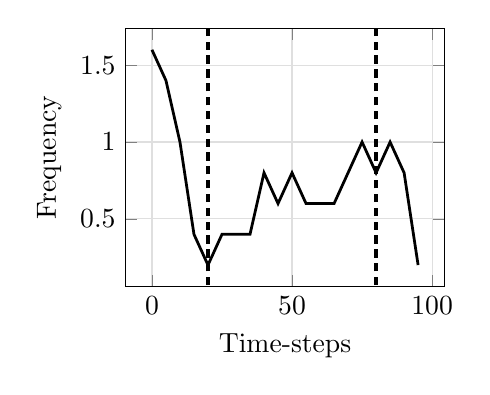
\begin{tikzpicture}
\begin{axis}[
    xlabel=Time-steps,
	ylabel= Frequency,
	title style={align=left},
	grid=both,
	minor grid style={gray!25},
	major grid style={gray!25},
	legend style={at={(1.0,1.05)},anchor=south east},
	width=0.465\linewidth,
	no marks
    ]
\addplot+[line width=1pt,solid,color=black] plot coordinates { (0, 1.6) (5, 1.4) (10, 1) (15, 0.4) (20, 0.2) (25, 0.4)(30, 0.4)(35, 0.4)(40, 0.8)(45, 0.6)(50, 0.8)(55, 0.6)(60, 0.6)(65, 0.6)(70, 0.8)(75, 1)(80, 0.8)(85, 1)(90, 0.8)(95, 0.2)};

\draw [densely dashed, line width=1.5pt] (20,-2) -- (20,2);
\draw [densely dashed, line width=1.5pt] (80,-2) -- (80,2);
\end{axis}
\end{tikzpicture}
}
\caption{Undirected actions: Evolution of the reputation according to agent $A$, and frequency of trade offers made by agent $A$.}
\end{figure}




\subsection{Testing directed actions}

The same set of experiments was conducted again, now using the concept of \textit{directed actions}. As discussed in \RefSec{sub:directedtest}, the design of the directed transition model has a significant impact on the performance of the RepNet agent. Two directed transition models of vastly different quality were proposed, and the results are described hereafter.

\subsubsection{Well-designed directed transition model}

Analogously to the previous section, \RefFig{subfig:paccept2} shows the evolution of agent $A$'s action distribution for agent $B$ in state $s = 2$, \RefFig{subfig:image2} displays the image $B$ has of $A$ and vice versa, \RefFig{subfig:rep2} shows the reputation of $A$ and $B$, and \RefFig{subfig:freq2} displays the tangible effects of these variables on $A$'s behavior. 

The well-designed transition model noticeably improves the performance of the RepNet agent. While the trajectories showcase the same key elements as in the previous section, the pace at which agent $A$ is able to adapt has greatly improved. As $B$ refuses the offers during the 20 first time-steps, its reputation decreases along with $A$'s self-reputation. The directed transition model was designed such that agent $A$ believes that its reputation must be good for $B$ to be willing to trade with $A$ (\RefFig{subfig:prof2} and \RefFig{subfig:prof4}). As such, $A$'s relatively poor-in-comparison self-reputation has an immediate effect on the \textit{value} it associates with action \texttt{trade\_with\_B} during the look-ahead search. Said differently, it quickly becomes more \textit{valuable} to pick a different action over \texttt{trade\_with\_B}. This explains the rash changes in $A$'s behavior at the start. Incidentally, agent $A$ is able to quickly increase the rate at which it attempts to trade with $B$ once it notices $B$'s willingness to trade. The average rate ends up topping off higher than without the use of directed transitions.

\begin{figure}[h]
\subfloat[Probability of $B$ accepting and refusing $A$'s trade offers, according to $A$]
{
\label{subfig:paccept2}
\begin{tikzpicture}
\begin{axis}[
	xlabel=Time-steps,
	ylabel= Probability,
	title style={align=left},
	grid=both,
	minor grid style={gray!25},
	major grid style={gray!25},
	legend style={at={(1.0,1.05)},anchor=south east},
	width=0.47\linewidth,
	no marks]
\addplot[line width=1pt,solid,color=black] %
	table[x=b,y=a,col sep=comma]{CSV/tradeABaccept2.csv};
\addlegendentry{$AD_A(B,2)(\texttt{accept})$};

\addplot[line width=1pt,dotted,color=black] %
	table[x=b,y=a,col sep=comma]{CSV/tradeABrefuse2.csv};
\addlegendentry{$AD_A(B,2)(\texttt{refuse})$};

\draw [densely dashed, line width=1.5pt] (20,-2) -- (20,2);
\draw [densely dashed, line width=1.5pt] (80,-2) -- (80,2);
\end{axis}
\end{tikzpicture}
}
\quad
\subfloat[Image agents $A$ and $B$ have of each other, according to $A$]
{
\label{subfig:image2}
\begin{tikzpicture}
\begin{axis}[
	xlabel=Time-steps,
	ylabel= Image,
	title style={align=left},
	grid=both,
	minor grid style={gray!25},
	major grid style={gray!25},
	legend style={at={(1.0,1.05)},anchor=south east},
	width=0.47\linewidth,
	no marks]
\addplot[line width=1pt,solid,color=black] %
	table[x=b,y=a,col sep=comma]{CSV/tradeABimgAB.csv};
\addlegendentry{$Img_A(B,A)$};

\addplot[line width=1pt,dotted,color=black] %
	table[x=b,y=a,col sep=comma]{CSV/tradeABimgBA.csv};
\addlegendentry{$Img_A(A,B)$};

\draw [densely dashed, line width=1.5pt] (20,-2) -- (20,2);
\draw [densely dashed, line width=1.5pt] (80,-2) -- (80,2);
\end{axis}
\end{tikzpicture}
}
\caption{Well-designed directed transition model: Evolution of the action distribution and image function, according to agent $A$.}
\end{figure}

\begin{figure}[h]
\subfloat[Reputation of agents $A$ and $B$, according to $A$]
{
\label{subfig:rep2}
\begin{tikzpicture}
\begin{axis}[
	xlabel=Time-steps,
	ylabel= Reputation,
	title style={align=left},
	grid=both,
	minor grid style={gray!25},
	major grid style={gray!25},
	legend style={at={(0.57,0.70)},anchor=south east},
	width=0.465\linewidth,
	no marks]
\addplot[line width=1pt,solid,color=black] %
	table[x=b,y=a,col sep=comma]{CSV/tradeABrepA.csv};
\addlegendentry{$REP_A(A)$};

\addplot[line width=1pt,dotted,color=black] %
	table[x=b,y=a,col sep=comma]{CSV/tradeABrepB.csv};
\addlegendentry{$REP_A(B)$};

\draw [densely dashed, line width=1.5pt] (20,-2) -- (20,2);
\draw [densely dashed, line width=1.5pt] (80,-2) -- (80,2);
\end{axis}
\end{tikzpicture}
}
\quad
\subfloat[Frequency of the trade offers made by $A$, measured in 5 time-step intervals]
{
\label{subfig:freq2}
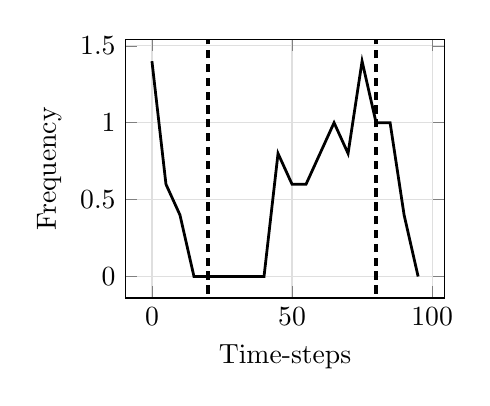
\begin{tikzpicture}
\begin{axis}[
    xlabel=Time-steps,
	ylabel= Frequency,
	title style={align=left},
	grid=both,
	minor grid style={gray!25},
	major grid style={gray!25},
	legend style={at={(1.0,1.05)},anchor=south east},
	width=0.465\linewidth,
	no marks
    ]
\addplot+[line width=1pt,solid,color=black] plot coordinates { (0, 1.4) (5, 0.6) (10, 0.4) (15, 0) (20, 0) (25, 0)(30, 0)(35, 0)(40, 0)(45, 0.8)(50, 0.6)(55, 0.6)(60, 0.8)(65, 1)(70, 0.8)(75, 1.4)(80, 1)(85, 1)(90, 0.4)(95, 0)};

\draw [densely dashed, line width=1.5pt] (20,-2) -- (20,2);
\draw [densely dashed, line width=1.5pt] (80,-2) -- (80,2);
\end{axis}
\end{tikzpicture}
}
\caption{Well-designed directed transition model: Evolution of the reputation according to agent $A$, and frequency of trade offers made by agent $A$.}
\end{figure}





\subsubsection{Poorly designed directed transition model}
The same set of experiments was conducted a third time with a poorly designed \textit{directed transition model}. As discussed in \RefSec{sub:directedtest}, the presently used directed transition model aims at making agent $A$ believe that agent $B$ will want to trade with $A$ in spite of a poor reputation. \RefFig{subfig:paccept3} displays the evolution of agent $A$'s action distribution for agent $B$, \RefFig{subfig:image3} shows the image $B$ has of $A$ and vice versa, \RefFig{subfig:rep3} shows the reputation of $A$ and $B$, and \RefFig{subfig:freq3} displays the tangible effects of these variables on $A$'s behavior.

The present experiment demonstrates that the presence of directed actions does not guarantee that the RepNet agent will perform better. In fact, a poorly designed directed transition model mitigates many of the benefits initially obtained by introducing the concepts of \textit{action distribution}, \textit{image}, and \textit{reputation}. In fact, the \textit{action distribution}, \textit{image}, and \textit{reputation} trajectories show that although the algorithm is capable of noticing the same changes in $B$'s behavior, the fact that it believes its reputation to be of little importance prevents it from adapting its own behavior. Consequently, agent $A$ has become slow at learning from other agents' behavior.
\begin{figure}[h]
\subfloat[Probability of $B$ accepting and refusing $A$'s trade offers, according to $A$]
{
\label{subfig:paccept3}
\begin{tikzpicture}
\begin{axis}[
	xlabel=Time-steps,
	ylabel= Probability,
	title style={align=left},
	grid=both,
	minor grid style={gray!25},
	major grid style={gray!25},
	legend style={at={(1.0,1.05)},anchor=south east},
	width=0.465\linewidth,
	no marks]
\addplot[line width=1pt,solid,color=black] %
	table[x=b,y=a,col sep=comma]{CSV/tradeABaccept2b.csv};
\addlegendentry{$AD_A(B,2)(\texttt{accept})$};

\addplot[line width=1pt,dotted,color=black] %
	table[x=b,y=a,col sep=comma]{CSV/tradeABrefuse2b.csv};
\addlegendentry{$AD_A(B,2)(\texttt{refuse})$};

\draw [densely dashed, line width=1.5pt] (20,-2) -- (20,2);
\draw [densely dashed, line width=1.5pt] (80,-2) -- (80,2);
\end{axis}
\end{tikzpicture}
}
\quad
\subfloat[Image agents $A$ and $B$ have of each other, according to $A$]
{
\label{subfig:image3}
\begin{tikzpicture}
\begin{axis}[
	xlabel=Time-steps,
	ylabel= Image,
	title style={align=left},
	grid=both,
	minor grid style={gray!25},
	major grid style={gray!25},
	legend style={at={(1.0,1.05)},anchor=south east},
	width=0.465\linewidth,
	no marks]
\addplot[line width=1pt,solid,color=black] %
	table[x=b,y=a,col sep=comma]{CSV/tradeABimgABb.csv};
\addlegendentry{$Img_A(B,A)$};

\addplot[line width=1pt,dotted,color=black] %
	table[x=b,y=a,col sep=comma]{CSV/tradeABimgBAb.csv};
\addlegendentry{$Img_A(A,B)$};

\draw [densely dashed, line width=1.5pt] (20,-2) -- (20,2);
\draw [densely dashed, line width=1.5pt] (80,-2) -- (80,2);
\end{axis}
\end{tikzpicture}
}
\caption{Poorly designed directed transition model: Evolution of the action distribution and image function, according to agent $A$.}
\end{figure}


\begin{figure}[h]
\subfloat[Reputation of agents $A$ and $B$, according to $A$]
{
\label{subfig:rep3}
\begin{tikzpicture}
\begin{axis}[
	xlabel=Time-steps,
	ylabel= Reputation,
	title style={align=left},
	grid=both,
	minor grid style={gray!25},
	major grid style={gray!25},
	legend style={at={(0.87,0.02)},anchor=south east},
	width=0.47\linewidth,
	no marks]
\addplot[line width=1pt,solid,color=black] %
	table[x=b,y=a,col sep=comma]{CSV/tradeABrepAb.csv};
\addlegendentry{$REP_A(A)$};

\addplot[line width=1pt,dotted,color=black] %
	table[x=b,y=a,col sep=comma]{CSV/tradeABrepBb.csv};
\addlegendentry{$REP_A(B)$};

\draw [densely dashed, line width=1.5pt] (20,-2) -- (20,2);
\draw [densely dashed, line width=1.5pt] (80,-2) -- (80,2);
\end{axis}
\end{tikzpicture}
}
\quad
\subfloat[Frequency of the trade offers made by $A$, measured in 5 time-step intervals]
{
\label{subfig:freq3}
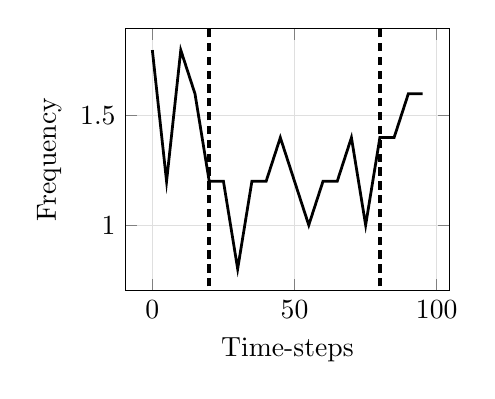
\begin{tikzpicture}
\begin{axis}[
    xlabel=Time-steps,
	ylabel= Frequency,
	title style={align=left},
	grid=both,
	minor grid style={gray!25},
	major grid style={gray!25},
	legend style={at={(1.0,1.05)},anchor=south east},
	width=0.47\linewidth,
	no marks
    ]
\addplot+[line width=1pt,solid,color=black] plot coordinates { (0, 1.8) (5, 1.2) (10, 1.8) (15, 1.6) (20, 1.2) (25, 1.2)(30, 0.8)(35, 1.2)(40, 1.2)(45, 1.4)(50, 1.2)(55, 1)(60, 1.2)(65, 1.2)(70, 1.4)(75, 1)(80, 1.4)(85, 1.4)(90, 1.6)(95, 1.6)};

\draw [densely dashed, line width=1.5pt] (20,-2) -- (20,2);
\draw [densely dashed, line width=1.5pt] (80,-2) -- (80,2);
\end{axis}
\end{tikzpicture}
}
\caption{Poorly designed directed transition model: Evolution of the reputation according to agent $A$, and frequency of trade offers made by agent $A$.}
\end{figure}



\section{Adaptability of the RepNet framework}
\label{sec:adapt}
As discussed in \RefSec{sub:adaptrep}, the present experiment aims at demonstrating the ability of the RepNet agent to adapt to changes in the behavior of another agent \textit{in the presence of imminent danger}. In this case, the danger comes in the form of aircraft crashes. Concretely the RepNet agent (agent $A$) is expected to be willing to sacrifice its own \textit{selfish} intentions to ensure no aircraft crashes occur. As a reminder, the selfishness of the second agent is increased every 10 time-steps. To show that the adaptations made by the RepNet agent are sound, the performance of the RepNet agent is compared to the performance of a classic MDP agent, i.e., an agent that does not adapt its behavior to fit the other agent's.

The first experiment of 15 runs was conducted to assess the ability of the RepNet agent to effectively reduce the number of crashes. \RefFig{subfig:crash} shows the evolution of the number of runs in which a crash has occurred as a function of the time-steps, for both the RepNet and MDP agents. It should be noted that these crashes can be inevitable. In fact, as the selfishness of the second agent increases, the probability of it deciding to stay at the vertiport when the RepNet agent's battery is low increases alongside. As such, an unfortunate sequence of steps, in which the second agent does not allow the RepNet agent to land when necessary will result in a crash regardless of the RepNet agent's actions.

The second experiment of 15 runs was conducted under the same circumstances, with the exception that the second agent never chooses to stay at the vertiport when the RepNet agent has little battery left. This makes it possible to uninterruptedly observe the adaptations made by the RepNet agent. \RefFig{subfig:timeground} displays the time the RepNet agent spends at the vertiport as a function of the time-steps.

The MDP agent's performance serves as a baseline. In particular, the graphs show that the RepNet agent is, on average, effectively able to \textit{delay} the time at which a crash occurs (\RefFig{subfig:crash}) by increasing the time it spends at the vertiport (\RefFig{subfig:timeground}). It thereby sacrifices its \textit{most} selfish intentions, which are to leave the vertiport when on the ground and leave the airspace when in the air, in an effort to avoid crashes.

\begin{figure}[h]
\subfloat[Number of runs in which a crash has occurred, as a function of the time-steps]
{
\label{subfig:crash}
\begin{tikzpicture}
\begin{axis}[
	xlabel=Time-steps,
	ylabel= {Number of crashes},
	title style={align=left},
	grid=both,
	minor grid style={gray!25},
	major grid style={gray!25},
	legend style={at={(1.0,1.05)},anchor=south east},
	width=0.48\linewidth,
	no marks]
\addplot[line width=1pt,solid,color=black] %
	table[x=b,y=a,col sep=comma]{CSV/vtol2crashes.csv};
\addlegendentry{RepNet-MDP};

\addplot[line width=1pt,dotted,color=black] %
	table[x=b,y=a,col sep=comma]{CSV/vtol2crashesmdp.csv};
\addlegendentry{MDP};

\draw [densely dashed, line width=1.5pt] (10,-2) -- (10,20);
\draw [densely dashed, line width=1.5pt] (20,-2) -- (20,20);
\draw [densely dashed, line width=1.5pt] (30,-2) -- (30,20);
\draw [densely dashed, line width=1.5pt] (40,-2) -- (40,20);
\end{axis}
\end{tikzpicture}
}
\quad
\subfloat[Average time agent $A$ spends on the ground, averaged over 10 time-steps]
{
\label{subfig:timeground}
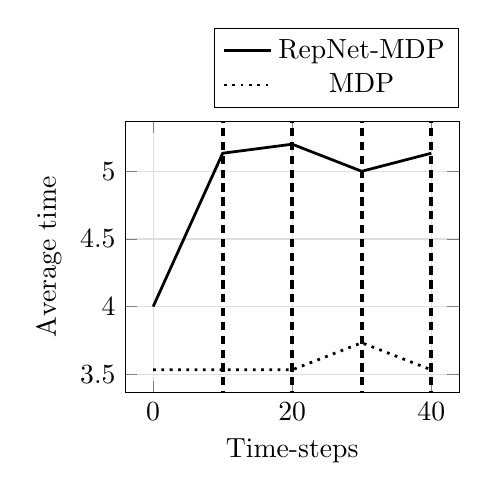
\begin{tikzpicture}
\begin{axis}[
	xlabel=Time-steps,
	ylabel= Average time,
	title style={align=left},
	grid=both,
	minor grid style={gray!25},
	major grid style={gray!25},
	legend style={at={(1.0,1.05)},anchor=south east},
	width=0.48\linewidth,
	no marks]
\addplot[line width=1pt,solid,color=black] %
	plot coordinates { (0, 4) (10, 5.133333333)(20, 5.2)(30, 5)(40, 5.133333333)};
\addlegendentry{RepNet-MDP};

\addplot[line width=1pt,dotted,color=black] %
	plot coordinates { (0, 3.533333333) (10, 3.533333333)(20, 3.533333333)(30, 3.733333333)(40, 3.533333333)};
\addlegendentry{MDP};

\draw [densely dashed, line width=1.5pt] (10,-2) -- (10,20);
\draw [densely dashed, line width=1.5pt] (20,-2) -- (20,20);
\draw [densely dashed, line width=1.5pt] (30,-2) -- (30,20);
\draw [densely dashed, line width=1.5pt] (40,-2) -- (40,20);
\end{axis}
\end{tikzpicture}
}
\caption{Number of crashes and average time spent at the vertiport by agent $A$.}
\end{figure}




\section{Large-scale experiments}
\label{sec:large}
To provide an initial understanding of the fundamental features that make up the RepNet framework, the number of agents was kept to 2 thus far. Increasing the number of agents aims at investing the robustness of the RepNet algorithm in the face of uncertainty. It also makes it possible to highlight potential deficiencies of the framework. As such, two large-scale experiments were set up to stress-test the multi-agent capabilities of the RepNet framework. \RefSec{sub:largetrade} investigates the ability of RepNet agents to draw conclusions on which actions to take based on other agents' actions that do not directly affect said RepNet agent. \RefSec{sub:largetaxi} explores the ability of several RepNet agents to cooperate in spite of their \textit{selfish} nature.

\subsection{Large-scale trading experiment}
\label{sub:largetrade}
The results of the 3-agent trading experiment are included in this section. The RepNet agent will be referred to as agent $A$ hereafter. The results have been averaged over 10 runs. \RefFig{subfig:rep3ag} shows the evolution of the reputations of agents $B$ and $C$. \RefFig{subfig:acc3ag} displays the evolution of the probabilities of agents $B$ and $C$ accepting trade offers from agent $A$. Finally, \RefFig{subfig:actiontaken} shows the average action taken by agent $A$ in the state in which the agents are allowed to make an offer.

Agent $B$ is told to refuse, and agent $C$ to accept, each trade offer during the first 33 time-steps. Expectedly, and in accordance with the results obtained in \RefSec{sec:feat}, agent $A$ is able to pick up on the other agents' behavioral habits as they directly affect it. As a result, the reputation of $B$ decreases, while the reputation of $C$ increases. All the while, agent $A$ chooses to conduct the majority of its trades with $C$.

The following 33 time-steps reverse $B$'s and $C$'s roles. Similarly, agent $A$ is able to adapt its behavior accordingly and ends up trading most of the time with $B$. The reputation of $B$ has increased, while the reputation of $C$ has decreased.

The interesting observations occur during the last 33 time-steps. Agents $B$ and $C$ are tasked with trading with one another. $B$ is asked to refuse all trade offers, while $C$ is asked to accept all trade offers. Here, Agent $A$'s actions have been blocked from having any effect on the environment. This is done in an effort to avoid that the RepNet agent can obtain direct feedback through its actions. It is thereby left with observing the trades that occur between agents $B$ and $C$. Unfortunately, the results show that even though the reputation of $B$ decreases and the reputation of $C$ increases according to $A$, the RepNet agent will still prefer to trade with $B$. In other words, as long as agent $A$ has not received direct confirmation from $B$ that it will refuse its \textit{own} offers, it will keep trying to trade with $B$ over Agent $C$.

The reason for this behavior is as follows: When agent $A$ performs a directed action targeted at another agent, say $B$, the result of the trade is, in the eyes of $A$, conditioned only by its own reputation (\RefSec{sec:reimagined}). Likewise, the probability of $B$ accepting (or refusing) $A$'s trade offer, according to $A$, is updated only through the direct experience it has with $B$ (as per \RefDef{def:actupnew}, and as can be seen in \RefFig{subfig:acc3ag}). The current implementation of the RepNet framework makes it impossible for Agent $A$ to learn from interactions it is not \textit{directly} affected by.

Whether this absence is to be seen as a shortcoming is up for debate. In fact, it may be desirable for a RepNet agent to require direct information before making up its mind, in an effort to avoid ill-informed decision-making. As an illustrative example, the fact that agent $B$ is refusing each trade offer from $C$ might just mean that $B$ believes $C$ to be unreliable; it might very well still be willing to trade with Agent $A$. On the other hand, this narrow-minded view on reputation noticeably mitigates the importance of said reputation as a whole.


\begin{figure}[h]
\subfloat[Reputation of agents $B$ and $C$, according to $A$]
{
\label{subfig:rep3ag}
\begin{tikzpicture}
\begin{axis}[
	xlabel=Time-steps,
	ylabel= Reputation,
	title style={align=left},
	grid=both,
	minor grid style={gray!25},
	major grid style={gray!25},
	legend style={at={(1.0,1.05)},anchor=south east},
	width=0.47\linewidth,
	no marks]
\addplot[line width=1pt,solid,color=black] %
	table[x=b,y=a,col sep=comma]{CSV/tradeABCrepB.csv};
\addlegendentry{$REP_A(B)$};

\addplot[line width=1pt,dotted,color=black] %
	table[x=b,y=a,col sep=comma]{CSV/tradeABCrepC.csv};
\addlegendentry{$REP_A(C)$};

\draw [densely dashed, line width=1.5pt] (33,-2) -- (33,2);
\draw [densely dashed, line width=1.5pt] (66,-2) -- (66,2);
\end{axis}
\end{tikzpicture}
}
\quad
\subfloat[Probability of agents $B$ and $C$ accepting trade offers from agent $A$, according to $A$]
{
\label{subfig:acc3ag}
\begin{tikzpicture}
\begin{axis}[
	xlabel=Time-steps,
	ylabel= Probability,
	title style={align=left},
	grid=both,
	minor grid style={gray!25},
	major grid style={gray!25},
	legend style={at={(1.0,1.05)},anchor=south east},
	width=0.47\linewidth,
	no marks]
\addplot[line width=1pt,solid,color=black] %
	table[x=b,y=a,col sep=comma]{CSV/tradeABCacceptB.csv};
\addlegendentry{$AD_A(B,\texttt{offer\_state})(\texttt{accept})$};

\addplot[line width=1pt,dotted,color=black] %
	table[x=b,y=a,col sep=comma]{CSV/tradeABCacceptC.csv};
\addlegendentry{$AD_A(C,\texttt{offer\_state})(\texttt{accept})$};

\draw [densely dashed, line width=1.5pt] (33,-2) -- (33,2);
\draw [densely dashed, line width=1.5pt] (66,-2) -- (66,2);
\end{axis}
\end{tikzpicture}
}
\caption{Evolution of the reputation of agents $B$ and $C$, and of the action distribution, according to agent $A$.}
\end{figure}




\begin{figure}[h]
\centering
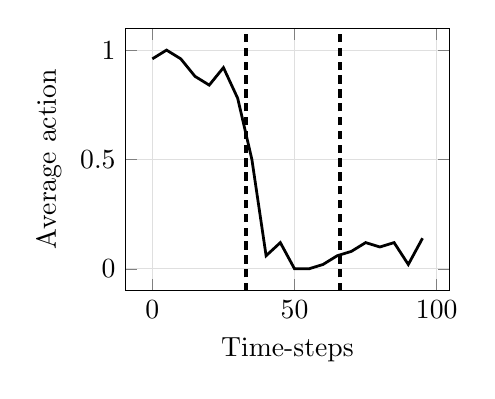
\begin{tikzpicture}
\begin{axis}[
	xlabel=Time-steps,
	ylabel= {Average action},
	grid=both,
	minor grid style={gray!25},
	major grid style={gray!25},
	legend style={at={(1.0,1.05)},anchor=south east},
	width=0.47\linewidth,
	no marks]
\addplot+[line width=1pt,solid,color=black] plot coordinates { (0, 0.96) (5, 1) (10, 0.96) (15, 0.88) (20, 0.84) (25,0.92)(30, 0.78)(35, 0.5)(40, 0.06)(45, 0.12)(50, 0)(55, 0)(60, 0.02)(65, 0.06)(70, 0.08)(75, 0.12)(80, 0.1)(85, 0.12)(90, 0.02)(95, 0.14)};
%\addlegendentry{Agent $A$};

%\addplot+[line width=1pt,dotted,color=black] plot coordinates { (0, 0.24) (5, 0.3) (10, 0.72) (15, 0.74) (20, 0.683333333) (25,0.6)(30, 0.666666667)(35, 0.38)(40, 0.38)(45, 0.36)(50, 0.2)(55, 0.26)(60, 0.32)(65, 0.5)(70, 0.54)(75, 0.44)(80, 0.48)(85, 0.54)(90, 0.46)(95, 0.525)};
%\addlegendentry{Q-Learner};

\draw [densely dashed, line width=1.5pt] (33,-2) -- (33,2);
\draw [densely dashed, line width=1.5pt] (66,-2) -- (66,2);
\end{axis}
\end{tikzpicture}
\caption{Average action taken by agent $A$, averaged over 5 time-steps. Action $a = 0$ corresponds to trading with agent $B$, action $a = 1$ corresponds to trading with agent $C$.}
\label{subfig:actiontaken}
\end{figure}

\subsection{Large-scale air-taxi experiment}
\label{sub:largetaxi}
In this final experiment, multiple RepNet agents are deployed in the same environment. In particular, 3 RepNet agents and 1 agent controlled by a simple algorithm have to find a way of reaching their goal destination (\textit{selfish} goal), whilst making sure crashes are avoided. As the \textit{non}-RepNet agent's selfishness increases every 20 time-steps, it becomes all the more important for each RepNet agent to find a balance between their most \textit{selfish} goal and the \textit{well-being} of the network as a whole. As discussed in \RefSec{sub:largeexp}, agents are redeployed randomly anytime they either all reach their goal destination of a crash occurs. The end goal for the RepNet agents is to minimize the number of crashes and simultaneously maximize the number of successful runs. 

\RefFig{subfig:crash22} depicts the frequency at which crashes occur, as a function of the time-steps. \RefFig{subfig:succ} shows the frequency at which the four agents manage to collectively reach their respective goal destinations. The graphs provide important insights into the ability of multiple RepNet agents to collectively adapt to the unpredictability of the \textit{non}-RepNet agent's behavior. As such, each increase in the selfishness of this agent is met by a peak in crashes and a drop in successful runs shortly after. This is to be expected as the RepNet agents can not predict the \textit{non}-RepNet agent's behavioral changes. Following each peak, the RepNet agents manage to each find a new stable policy that allows each agent to reach their goal destination safely. The frequency of successful runs increases until the next increase in the selfishness of the \textit{non}-RepNet agent. The ability of the RepNet agents to collectively \textit{converge} to a stable situation is not trivial. \RefSec{sec:additional} briefly discussed the convergence problem inherently present in \textit{Multi-agent learning} (MAL). While \textit{Single-agent learning} (SAL) algorithms are often able to provide certain convergence guarantees, the same can not be said of MAL algorithms \cite{nonstation, convergence}. Concretely, the convergence of one agent's policy is a function of the behavior of all other agents in the network. This makes it all the more interesting that given a properly tuned set of parameters, RepNet agents are able to come to a mutual agreement that benefits the entire network. It should be noted here that the topic of convergence in MAL is vastly more complex than can be summarized in a single experiment \cite{reduce, reduce2, nonstation, convergence}. The present experiment merely provides encouraging results as to the viability of the RepNet framework.


\begin{figure}[h]
\subfloat[Frequency of crashes]
{
\label{subfig:crash22}
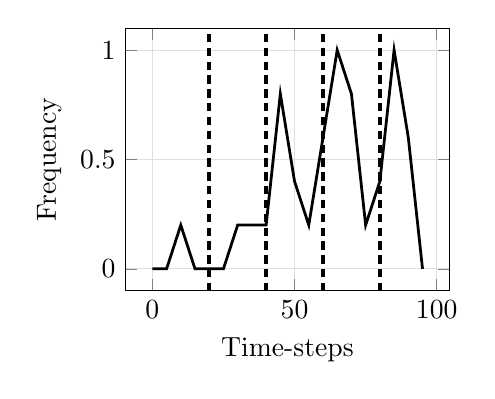
\begin{tikzpicture}
\begin{axis}[
    xlabel=Time-steps,
	ylabel= Frequency,
	title style={align=left},
	grid=both,
	minor grid style={gray!25},
	major grid style={gray!25},
	legend style={at={(1.0,1.05)},anchor=south east},
	width=0.47\linewidth,
	no marks
    ]
\addplot+[line width=1pt,solid,color=black] plot coordinates { (0, 0) (5, 0) (10, 0.2) (15, 0) (20, 0) (25,0)(30, 0.2)(35, 0.2)(40, 0.2)(45, 0.8)(50, 0.4)(55, 0.2)(60, 0.6)(65, 1)(70, 0.8)(75, 0.2)(80, 0.4)(85, 1)(90, 0.6)(95, 0)};
\draw [densely dashed, line width=1.5pt] (20,-2) -- (20,2);
\draw [densely dashed, line width=1.5pt] (40,-2) -- (40,2);
\draw [densely dashed, line width=1.5pt] (60,-2) -- (60,2);
\draw [densely dashed, line width=1.5pt] (80,-2) -- (80,2);
\end{axis}
\end{tikzpicture}
}
\subfloat[Frequency of successful runs]
{
\label{subfig:succ}
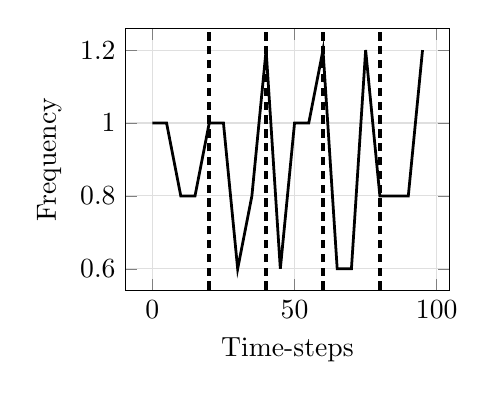
\begin{tikzpicture}
\begin{axis}[
    xlabel=Time-steps,
	ylabel= Frequency,
	title style={align=left},
	grid=both,
	minor grid style={gray!25},
	major grid style={gray!25},
	legend style={at={(1.0,1.05)},anchor=south east},
	width=0.47\linewidth,
	no marks
    ]
\addplot+[line width=1pt,solid,color=black] plot coordinates { (0, 1) (5, 1) (10, 0.8) (15, 0.8) (20, 1) (25,1)(30, 0.6)(35, 0.8)(40, 1.2)(45, 0.6)(50, 1)(55, 1)(60, 1.2)(65, 0.6)(70, 0.6)(75, 1.2)(80, 0.8)(85, 0.8)(90, 0.8)(95, 1.2)};
\draw [densely dashed, line width=1.5pt] (20,-2) -- (20,2);
\draw [densely dashed, line width=1.5pt] (40,-2) -- (40,2);
\draw [densely dashed, line width=1.5pt] (60,-2) -- (60,2);
\draw [densely dashed, line width=1.5pt] (80,-2) -- (80,2);
\end{axis}
\end{tikzpicture}
}
\caption{Frequency of crashes and successful runs during the 4-agent air-taxi experiment, averaged over 5 time-steps.}
\end{figure}





\section{Summary of the results}
\label{sec:summa}


The first part of the experimental setup has shown the RepNet algorithm to be able to leverage the notions of \textit{action distribution}, \textit{image}, and \textit{reputation} to aid in its decision-making process, in the presence of a second agent. The concept of \textit{directed actions} was shown to be effective, provided that the corresponding \textit{directed transition model} was carefully designed. Failing to do so resulted in the RepNet agent barely being able to learn.
The second part demonstrated the ability of the RepNet to partially sacrifice its \textit{selfish} goal in an effort to prevent crashes from occurring. 
The large-scale trading example highlighted a potential shortcoming of the current version of the RepNet algorithm. In fact, the algorithm is unable to learn from experiences that do not affect it directly. 
Finally, the large-scale aircraft example showcases the possibility of several RepNet agents to be deployed in the same environment and having them cooperate with one another. It provides early results as to the convergence properties of well-tuned RepNet agents.